\documentclass[t, 10pt, aspectratio=169, table, x11names]{beamer}
\usetheme{metropolis}

\usepackage{xcolor}
\usepackage[utf8]{inputenc}
\usepackage[default]{lato}
\usepackage[T1]{fontenc}
\usepackage{lmodern}
\usepackage{listingsutf8}
\usepackage{hyperref}
\usepackage{wrapfig}
\usepackage{dsfont}
\usepackage[export]{adjustbox}
\usepackage{array, booktabs}
\usepackage{cellspace}

\graphicspath{{./resources}}
\lstset{inputpath=./resources, xleftmargin=7mm, xrightmargin=7mm}

\definecolor{codegreen}{rgb}{0,0.6,0}
\definecolor{codegray}{rgb}{0.5,0.5,0.5}
\definecolor{codepurple}{rgb}{0.58,0,0.82}
\definecolor{backcolour}{rgb}{0.95,0.95,0.92}
\hypersetup{colorlinks,urlcolor=blue}

\newcommand{\redhighlight}[1]{{\color{red}\textbf{\texttt{#1}}}}

\newcommand{\R}{\mathds{R}}
\newcommand{\appallingunderline}[1]{
	\underline{\smash{#1}\vphantom{T}}\vphantom{#1}%
}

\lstdefinestyle{sql}{
	backgroundcolor=\color{backcolour},
	commentstyle=\color{codegreen},
	keywordstyle=\color{magenta},
	numberstyle=\tiny\color{codegray},
	stringstyle=\color{codepurple},
	basicstyle=\ttfamily\scriptsize,
	breakatwhitespace=false,
	breaklines=true,
	captionpos=b,
	keepspaces=true,
	numbers=left,
	numbersep=5pt,
	showspaces=false,
	showstringspaces=false,
	showtabs=false,
	tabsize=2
}

\lstdefinestyle{winprompt}{
	backgroundcolor=\color{backcolour},
	commentstyle=\color{codegreen},
	keywordstyle=\color{magenta},
	numberstyle=\tiny\color{codegray},
	stringstyle=\color{codepurple},
	basicstyle=\ttfamily\footnotesize,
	breakatwhitespace=false,
	breaklines=false,
	breakatwhitespace=false,
	prebreak=false,
	captionpos=b,
	keepspaces=true,
	showspaces=false,
	showstringspaces=false,
	showtabs=false,
	tabsize=1
}

\lstset{style=sql}
\lstset{inputencoding=utf8/latin1}


\begin{document}

	%Author, Title and subtitle
	\author{Victor Mayrink}
	\title{Curso de SQL}
	\subtitle{Aula 0: Introdução e motivação}

	%Fame: title
	\begin{frame}[plain]
		\maketitle
	\end{frame}
	
	%Frame: agenda
	\begin{frame}
		\frametitle{Agenda}
		\vspace{1cm}
		\begin{enumerate}
			\large
			\item O que é SQL
			\item Por quê aprender SQL?
			\item Instalação e configuração das ferramentas
		\end{enumerate}
	\end{frame}
	
	%Frame: sql meaning
	\begin{frame}
		\frametitle{O que é SQL?}
		\vspace{0.3cm}
		\begin{itemize}
			\setlength{\itemsep}{8pt}
			\item A sigla SQL significa \textbf{\textit{Structured Query Language}}
			\item Beleza, mas que \textit{diabos} é isso?
			\vspace{5mm}
			\begin{figure}[h]
				\fbox{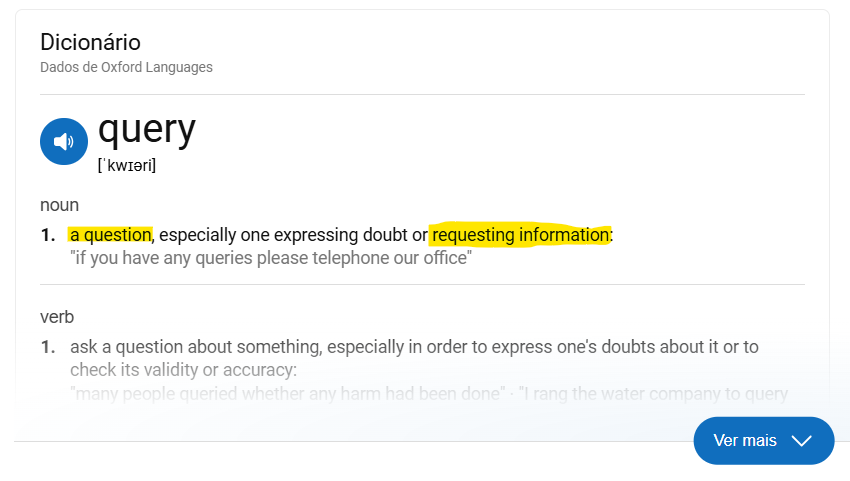
\includegraphics[width=0.55\textwidth]{query-meaning.png}}
			\end{figure}
		\end{itemize}
	\end{frame}

	%Frame: questions are more important than answers
	\begin{frame}
		\frametitle{O que é SQL?}
		\vspace{2mm}
		\begin{itemize}
			\setlength{\itemsep}{8pt}
			\item SQL é uma linguagem para \textit{fazer \textbf{perguntas} à um banco de dados}
		\end{itemize}
		\vspace{2mm}
		\begin{figure}[h]
			
\includegraphics[height=40mm]{voltaire.jpg}
			\hspace{5mm}
			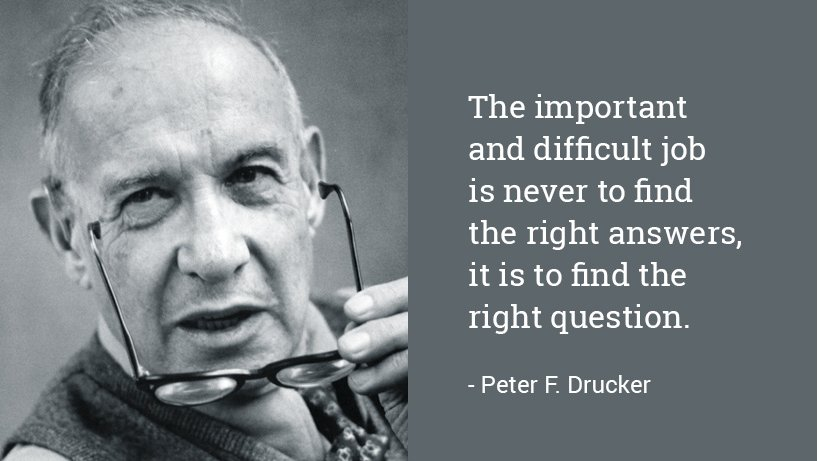
\includegraphics[height=40mm]{peter-drucker.jpg}
		\end{figure}
	\end{frame}

	%Frame: sql usage
	\begin{frame}
		\frametitle{O que é SQL?}
		\vspace{0.3cm}
		\begin{itemize}
			\setlength{\itemsep}{8pt}
			\item Estritamente falando, o SQL não serve \textit{\textbf{somente}} para fazer perguntas. 
			\item O SQL é a linguagem mais utilizada para executar comandos em um banco de dados
			\vspace{0.11cm}
			\begin{itemize}
				\item criar tabelas,
				\item inserir novos registros,
				\item atualizar registros existentes,
				\item excluir registros,
				\item etc... (veremos mais adiante)
			\end{itemize}
			\vspace{0.5cm}
			\begin{center}
				No entanto, o SQL é utilizado principalmente para realizar \textit{consultas} no banco.\\
				Ou seja, \textbf{fazer perguntas}.
			\end{center}
		\end{itemize}
	\end{frame}

	%Frame: why you should learn SQL
	\begin{frame}
		\frametitle{Por quê aprender SQL?}
		\vspace{2mm}
		\begin{itemize}[<+->]
			\setlength{\itemsep}{7pt}
			\item SQL é uma habilidade \textit{muito valorizada} no mercado
			\item Conhecer SQL é útil para profissionais de \textit{diversas especialidades}
			\item SQL é uma \textit{linguagem universal} para bancos de dados relacionais.
			\item O entendimento de como os dados da sua empresa estão organizados contribui para que os profissionais tenham uma \textit{visão mais sistêmica do negócio} e dos processos operacionais.
			\item \textit{Individualmente}, o conhecimento de SQL contribuí para a capacidade analítica do profissional
			\item \textit{Coletivamente}, o uso extensivo de SQL entre os profissionais de uma empresa contribui para a criação de uma cultura orientada a dados e resultados
		\end{itemize}
	\end{frame}
	
	\section{Vamos começar}
	
	%Frame: doctor scheduling example
	\begin{frame}
		\frametitle{Registro de dados}
		\vspace{3mm}
		Imagine um formulário para fazer o agendamento de uma consulta médica...
		\begin{columns}[t]
			\begin{column}{0.50\textwidth}
				\vspace{0.3cm}
				\begin{figure}[h]
					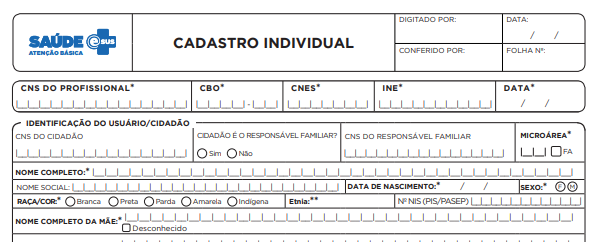
\includegraphics[width=63mm, right]{sample-form.png}
				\end{figure}
			\end{column}
			\begin{column}{0.53\textwidth}
				\begin{itemize}					
					\item O formulário possui diversos \textit{\textbf{campos}} que devem ser preenchidos
					\vspace{2mm}
					\item Cada campo do formulário armazena um determinado \textit{\textbf{tipo de dado}}
					\vspace{2mm}
					\begin{itemize}
						\ttfamily\small
						\item Nome: texto
						\item Data de nascimento: data
						\item Peso e altura: numérico
						\item Possui comorbidades: sim/não
						\item Agendamento: data e horário
					\end{itemize}
				\end{itemize}
			\end{column}
			\begin{column}{0.05\textwidth}
			\end{column}
		\end{columns}
	\end{frame}
	
	%Frame: rows and columns
	\begin{frame}
		\frametitle{Registro de dados}
		\vspace{3mm}
		As fichas do formulário podem ser armazenadas em uma tabela 
		\begin{itemize}
			\item Cada ficha preenchida torna-se uma \textbf\textit{linha} ou \textbf{\textit{registro}} na tabela
			\item Os campos do formulário tornam-se \textbf{\textit{colunas}} na tabela
		\end{itemize}		
	\end{frame}
	
	%Frame: insert
	\begin{frame}
		\frametitle{Registro de dados}
		Alguns dados fictícios (gerados pelo ChatGPT)
		\begin{table}[ht]
			\centering
			\footnotesize
			\begin{tabular}{|l|l|l|l|l|}
				\hline
				\rowcolor{SeaGreen3!30!}
				\textbf{nome\_paciente} & \textbf{data\_nasc\_paciente} & \textbf{nome\_medico} & \textbf{especialidade\_medico} & \textbf{data\_hora\_consulta} \\
				\hline
				Alice Oliveira & 12/03/1979 & Dr. Martins & Cardiologia & 18/07/2024 10:00 \\
				\hline
				Alice Oliveira & 12/03/1979 & Dra. Santos & Dermatologia & 22/07/2024 15:30 \\
				\hline
				Carlos Souza & 05/08/1985 & Dr. Almeida & Ortopedia & 05/06/2024 08:45 \\
				\hline
				Carlos Souza & 05/08/1985 & Dra. Lima & Pediatria & 12/06/2024 14:00 \\
				\hline
				Maria Silva & 30/11/1967 & Dr. Pereira & Oftalmologia & 10/07/2024 09:15 \\
				\hline
				Maria Silva & 30/11/1967 & Dra. Costa & Ginecologia & 18/07/2024 11:00 \\
				\hline
				João Santos & 20/04/1992 & Dr. Almeida & Neurologia & 02/08/2024 16:30 \\
				\hline
				João Santos & 20/04/1992 & Dra. Lima & Endocrinologia & 09/08/2024 08:00 \\
				\hline
				Luana Oliveira & 15/09/1988 & Dr. Costa & Urologia & 15/06/2024 13:45 \\
				\hline
				Luana Oliveira & 15/09/1988 & Dra. Santos & Psiquiatria & 25/06/2024 10:30 \\
				\hline
				Rafaela Lima & 03/07/1983 & Dr. Martins & Oftalmologia & 20/07/2024 14:15 \\
				\hline
				Rafaela Lima & 03/07/1983 & Dra. Costa & Dermatologia & 28/07/2024 09:45 \\
				\hline
				Pedro Almeida & 10/10/1975 & Dr. Pereira & Cardiologia & 05/08/2024 11:30 \\
				\hline
				Pedro Almeida & 10/10/1975 & Dra. Santos & Pediatria & 12/08/2024 15:00 \\
				\hline
			\end{tabular}
		\end{table}
	\end{frame}
	
	%Frame: create table
	\begin{frame}
		\frametitle{Criação da tabela no SQL}
		Para criar uma tabela como essa, utilizamos o comando \bluehighlight{CREATE TABLE}:
		\lstinputlisting[language=Sql]{table-consultas-create-1.sql}
		Vamos analisar a estrutura desse comando:
		\lstinputlisting[language=Sql]{table-consultas-create-2.sql}
	\end{frame}	
	
	%Frame: insert records
	\begin{frame}
		\frametitle{Inserir registros na tabela}
		Para inserir registros, utilizamos o comando \bluehighlight{INSERT INTO ... VALUES}:
		\lstinputlisting[language=Sql, xleftmargin=0mm, xrightmargin=0mm]{table-consultas-ingest-1.sql}
	\end{frame}

	%Frame: select
	\begin{frame}
		\frametitle{Consultar registros}
		Para consultar os registros de uma tabela, usamos o comando \bluehighlight{SELECT}.
		\lstinputlisting[language=Sql]{table-consultas-select-1.sql}
		Resposta do servidor:
		\lstinputlisting[language=Sql]{table-consultas-select-1-result.sql}
	\end{frame}

	%Frame: practical case
	\begin{frame}
		\frametitle{Exemplo prático com o Dbeaver}
		Para consultar os registros de uma tabela, usamos o comando \bluehighlight{SELECT}.
		\lstinputlisting[language=Sql]{table-consultas-select-1.sql}
		Resposta do servidor:
		\lstinputlisting[language=Sql]{table-consultas-select-1-result.sql}
	\end{frame}
	
	%Frame: update
	\begin{frame}
		\frametitle{Atualizar registros}
		Para atualizar os registros de uma tabela, usamos o comando \bluehighlight{UPDATE...SET} 
		\lstinputlisting[language=Sql]{table-consultas-update-1.sql}
		Se fizermos a consulta novamente
		\lstinputlisting[language=Sql]{table-consultas-select-1.sql}
		\lstinputlisting[language=Sql]{table-consultas-select-1-result-2.sql}
	\end{frame}
	
	%Frame: delete
	\begin{frame}
		\frametitle{Deletar registros}
		Para apagar um registro utilizamos o comando \bluehighlight{DELETE}
		\lstinputlisting[language=Sql]{table-consultas-delete-1.sql}
	\end{frame}
	
\end{document}